\documentclass[10pt, a4paper]{article}

% On écrit en français
\usepackage[utf8]{inputenc}
\usepackage[frenchb]{babel}
\usepackage[T1]{fontenc}

% Packages nécessaires
\usepackage{graphicx}
\usepackage{hyperref}

% Numérotation de page custom
\usepackage{fancyhdr}
\usepackage{lastpage}
\pagestyle{fancy}
\fancyhf{}
\rfoot{Page \thepage \hspace{1pt} sur \pageref{LastPage}}

% Police Helvetica <3
\usepackage{helvet}
\renewcommand*{\familydefault}{\sfdefault}

% Enlever les alinéas
\setlength{\parindent}{0pt}

% Marges plus larges pour faire moins LaTeX
\usepackage[left=3cm, right=3cm]{geometry}

% Sous titre de document
\usepackage{titling}
\newcommand{\subtitle}[1]{%
  \posttitle{%
    \par\end{center}
    \begin{center}\large#1\end{center}
    \vskip0.5em}%
}

% En tête complet de document
\newcommand{\Document}[1]{%
    \title{#1}
    \subtitle{Dématérialisation d'un processus de paiement}
    \author{
        COMETS Jean-Marie \\
        DELMARRE Adrian \\
        REYNOLDS Nicolas \\
        TURPIN Pierre
    }
    \date{\today}

    \maketitle \newpage

    \tableofcontents \newpage
}


\begin{document}

\Document{Dossier d'initialisation}

\section{Contexte et objet du projet}

Les offres de "titre-restaurant" existent depuis le début des années 1960, et
le groupe Sodexo est le seul sur le marché des chèques restaurant depuis 1987.
De plus, de nombreux restaurants d'entreprise sont déjà gérés par Sodexo. C'est
donc un leader ancré sur le marché. \\

L'entreprise Aventix souhaite concurrencer l'offre de Sodexo en remplaçant les
chèques restaurant par un système entièrement dématérialisé. \\

Le projet se situe donc au coeur de la numérisation du contenu, l'évolution des
systèmes existants vers des "modèles virtuels", réduisant ainsi l'utilisation
de papier et offrant de nouvelles possibilités d'interfaçage. \\

L'objet du projet est donc d'établir une offre technico-commerciale de solution
de ticket restaurant numérique. L'ensemble des attentes émises et les solutions
envisagées seront détaillées dans le document "Expression des besoins", livré
au cours de la deuxième phase du projet.

\section{Description des livrables}
\begin{description}
    \item[Dossier d'initialisation] ce document, fourni dès l'entame du projet.
    \item[Plan d'Assurance Qualité (PAQ)] rendu avec chaque nouveau rendu de
        livrable, relatant la structure détaillée des livrables ainsi que les
        méthodes employés pour garantir leur qualité. Un glossaire est
        notamment inclus pour assurer la bonne compréhension des documents.
        Chaque nouvelle modification impacte les nouveaux livrables ou
        exceptionnellement ceux qui ont dû être modifiés après vérification de
        la part du client.
    \item[Expression des besoins] description de la solution demandée et mise en
        rapport avec la solution envisagée, ainsi que benchmarking des solution
        de paiement et de leur interconnexion avec un SI.
    \item[Architecture applicative] urbanisation du SI et architecture des services mis en jeu.
    \item[Architecture technique] moyens techniques envisagés pour le déploiement de la solution.
    \item[Business plan] définition des objectifs, description de l'organisation
        existante et des moyens à mettre en oeuvre pour atteindre les objectifs
        fixés.
\end{description}

\section{Gestion de projet}

La gestion de projet sera basée sur un modèle agile, avec des \textit{sprints}
d'une semaine. Chaque semaine, une réunion d'équipe est prévue, avec le
planning suivant :

\begin{enumerate}
    \item Bilan de la semaine passée, avancement actuel de chacun
    \item Risques déduits de l'avancement
    \item Remarques variées sur l'état des livrables déjà produits,
        propositions d'améliorations
    \item Définition des tâches à effectuer pour la semaine à venir
    \item Pré-attribution en rapport avec les anciennes responsabilités de
        chacun
    \item Notation collaborative des tâches par difficulté (chacun note
        séparément, puis moyenne des notes)
    \item Ré-attribution des tâches pour équilibrer la charge de travail
        (basculement des responsabilités)
    \item Réflexion d'équipe sur les tâches les plus difficiles (une voire deux
        en fonction du temps disponible)
\end{enumerate}

En cas de force majeure rendant indisponible un membre de l'équipe, une réunion
exceptionnelle peut être planifiée pour redistribuer les tâches de ce dernier.

\section{Organisation de l'équipe}

L'organisation hiérarchique de l'équipe est détaillée dans la figure
\ref{fig:hierarchie}, mais peut être résumée comme ceci :

\begin{itemize}
    \item Jean-Marie Comets (chef de projet)
    \item Pierre Turpin (responsable qualité)
    \item Adrian Delmarre
    \item Nicolas Reynolds
\end{itemize}

L'ensemble des membres de l'équipe sont en dernière année de formation d'école
d'ingénieurs à l'INSA de Lyon. C'est une équipe motivée et passionnée
d'innovation.

\begin{figure}[!htb]
    \centering
    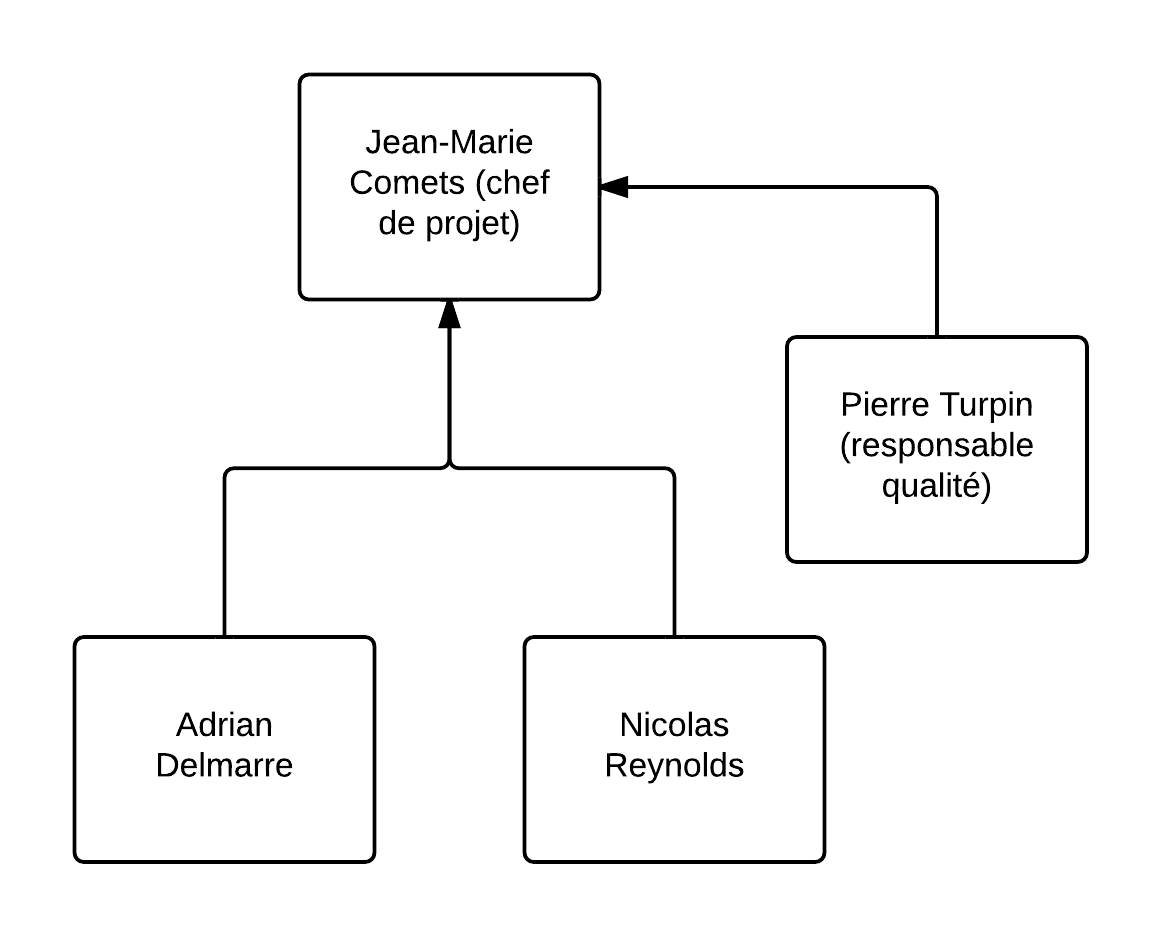
\includegraphics[width=0.8\textwidth]{hierarchie}
    \caption{Hiérarchie de l'équipe}
    \label{fig:hierarchie}
\end{figure}

\section{Analyse des risques}

\subsection{Facteurs de risque}

\begin{description}
    \item[Difficultés techniques] La spécificité du domaine d'étude demande une
        forte spécialisation des membres de l'équipe.
    \item[Degré d'intégration et taille du projet] Le projet est ambitieux et
        complexe. Son envergure laisse présager une architecture modulaire
        entraînant des dépendances et interactions fortes. Une forte rigueur
        organisationnelle sera nécessaire, et on peu envisager le recours à des
        méthodes de développement Agile (de type Scrum).
    \item[Instabilité de l'équipe] Une émulation mutuelle est nécessaire pour
        prévenir une éventuelle démotivation de l'équipe.
\end{description}

\subsubsection{Configuration organisationnelle}

\begin{description}
    \item[Travail collaboratif] Mise en place de normes, d'un guide de style,
        de chartes graphiques et d'outils collaboratifs.  Définition du
        workflow-type du cycle de production et de validation d'un livrable.
    \item[Echéances] Il est impératif de mettre en place un suivi régulier de
        la planification et d'un échéancier large. Le chef de projet et le
        responsable qualité doivent veiller régulièrement au respect des
        échéances et anticiper les suivantes.
\end{description}

\subsection{Risques liés au projet}

\begin{description}
    \item[Risques financiers] En l'occurrence, il s'agira principalement de
        dépassement de volume raisonnable de travail.  Il incombe au chef de
        projet de mener à bien une planification stricte structurée par un
        suivi régulier du temps de travail sur chaque tâche. Il sera nécessaire
        de prévoir des indicateurs significatifs de ces aspects sur les
        tableaux de bord de suivi de projet.
    \item[Risques humains] D'éventuels cas d'incompétence seront prévenus par
        l'allocation de créneaux de veille technologique, et le recours
        systématique à l'entraide.
    \item[Risques technologiques] Pour prévenir la perte de documents, un
        gestionnaire de version sera systématiquement utilisé.
\end{description}

\end{document}

% vim: ft=tex et sw=4 sts=4
